\documentclass{article}

\usepackage{graphicx}
\usepackage{tikz}
\usepackage{tikzsymbols}
\usetikzlibrary{calc,patterns,shapes.geometric}
\pagestyle{empty}
\usepackage[margin=0pt]{geometry}
\geometry{papersize={14in,12in}}

\def\centerarc[#1](#2)(#3:#4:#5){\draw[#1] ($(#2)+({#5*cos(#3)},{#5*sin(#3)})$) arc (#3:#4:#5);}

\begin{document}
	\begin{figure}
		\centering
		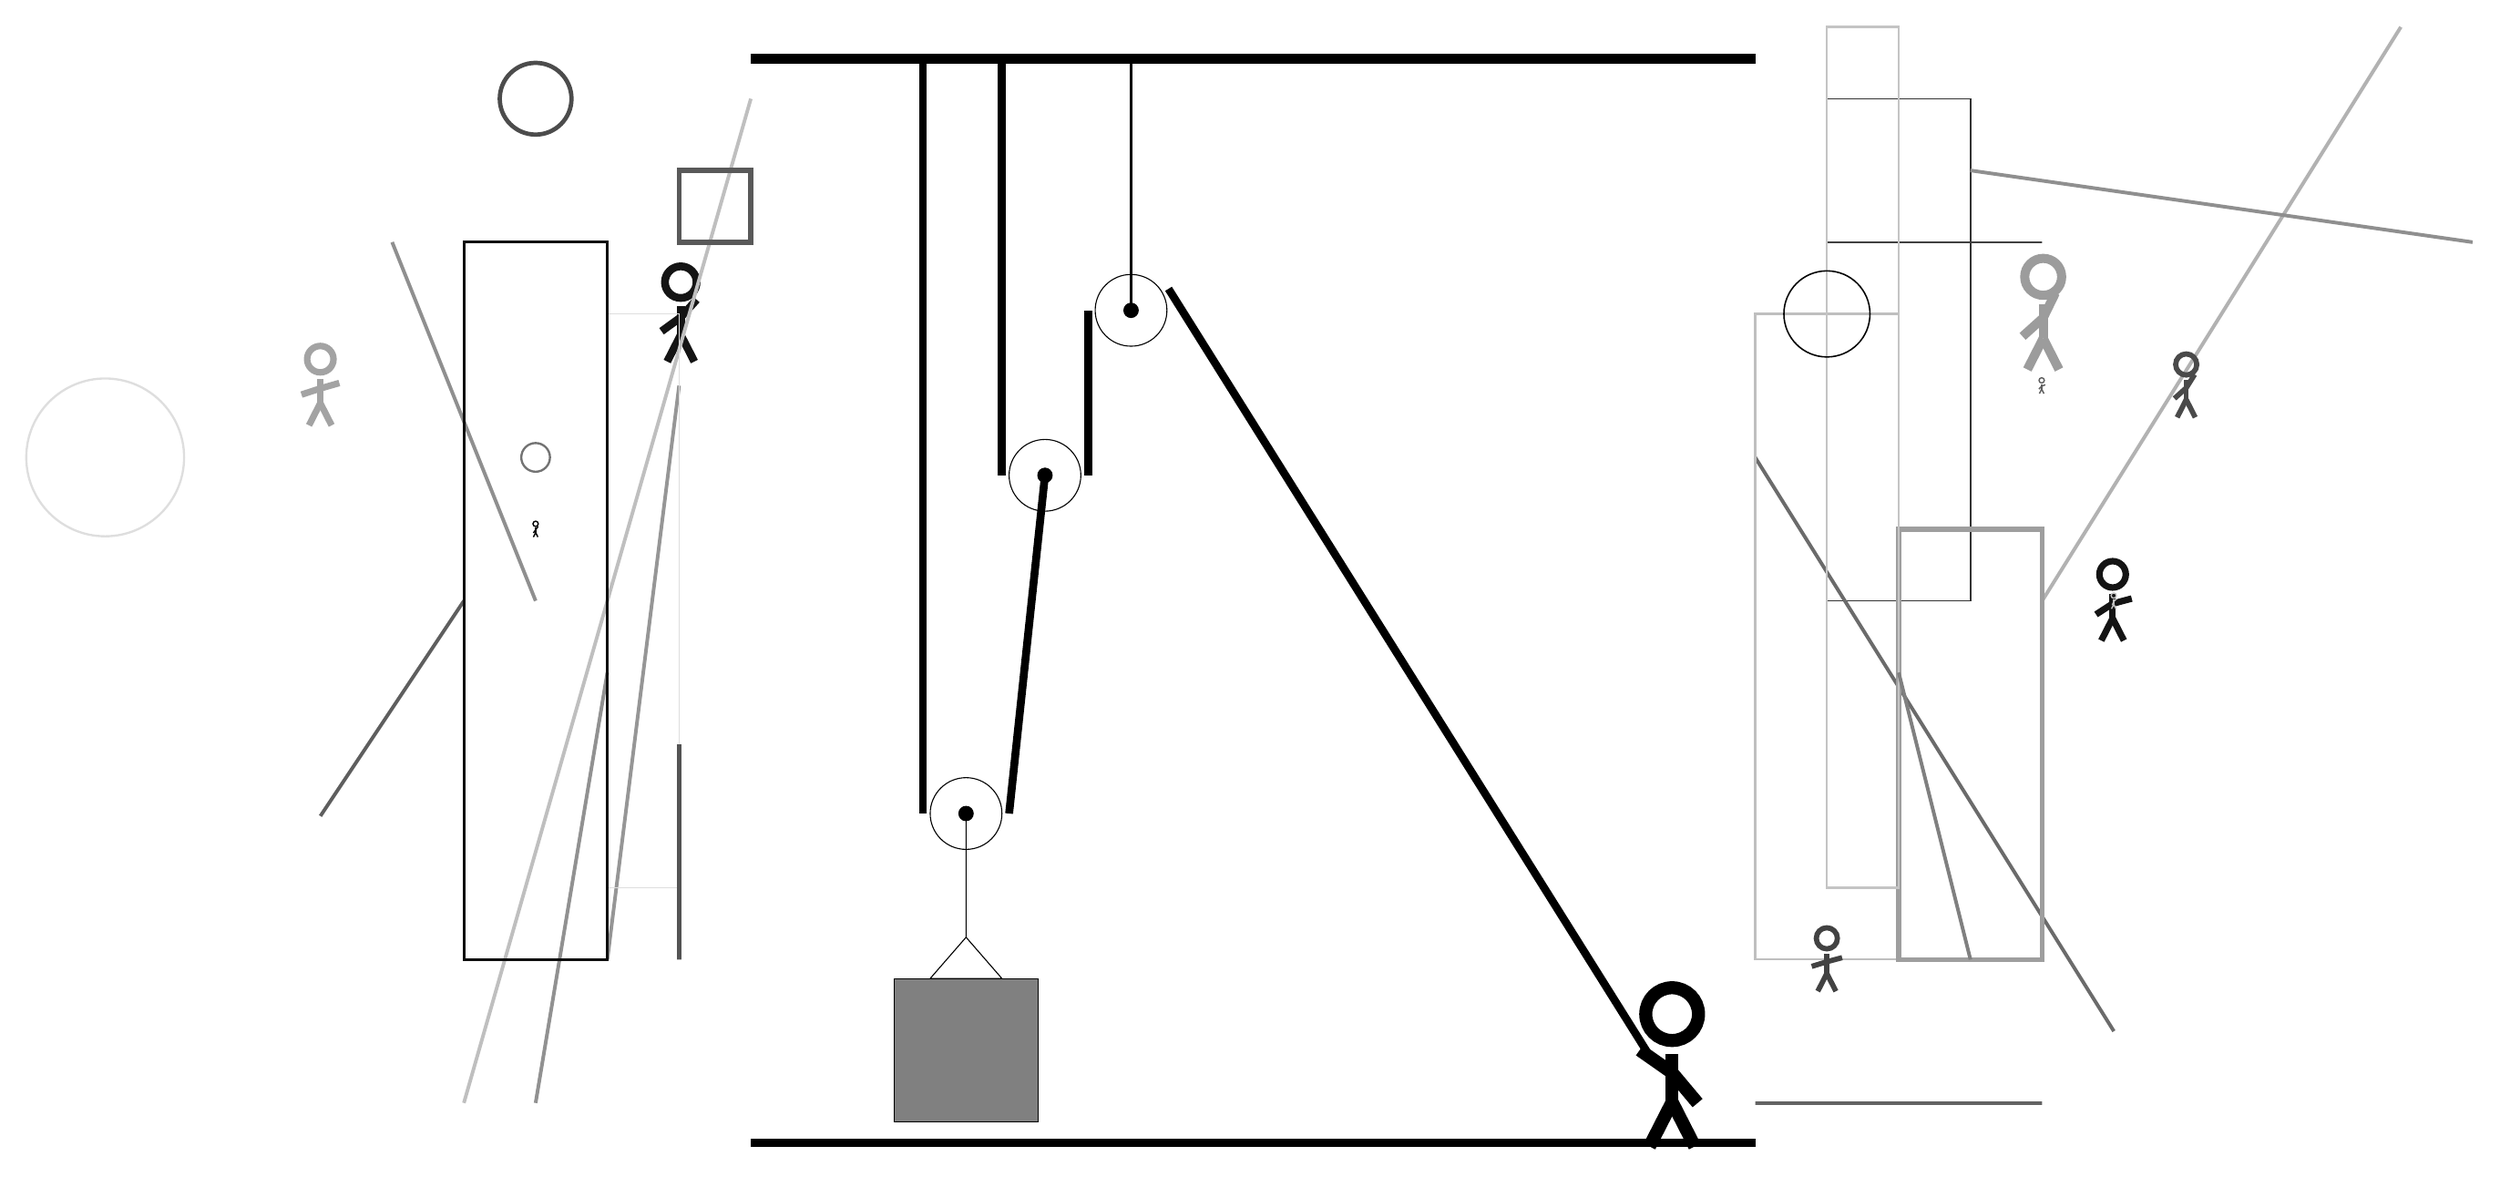
\begin{tikzpicture}
			%%%%% START %%%%%
			
			\draw[fill=black] (-2, 11.5) rectangle (12, 11.625);
			
			\node[line width=0.7mm, color=black!100] at (-5, 5) {\Strichmaxerl[1][56][52]};
			
			\draw[line width=0.5mm, color=black!44](-7, 9) -- (-5, 4);
			\draw[line width=0.5mm, color=black!63](-6, 4) -- (-8, 1);
			\draw[line width=0.5mm, color=black!41](-3, 7) -- (-4, -1);
			
			\node[line width=0.6mm, color=black!39] at (16, 8) {\Strichmaxerl[7][42][64]};
			\draw[line width=0.5mm, color=black!30](16, 4) -- (21, 12);
			\node[line width=0.6mm, color=black!63] at (16, 7) {\Strichmaxerl[1][46][22]};
			\node[line width=0.7mm, color=black!36] at (-8, 7) {\Strichmaxerl[5][18][16]};
			\draw[line width=0.5mm, color=black!43](-5, -3) -- (-4, 3);
			\node[line width=0.5mm, color=black!92] at (-3, 8) {\Strichmaxerl[6][36][48]};
			
			\draw[line width=0.5mm, color=black!25](-6, -3) -- (-2, 11);
			\node[line width=0.3mm, color=black!71] at (18, 7) {\Strichmaxerl[4][42][58]};
			\draw[line width=0.2mm, color=black!80] (13, 4) rectangle (15, 11);
			
			\draw [line width=0.6mm, color=black!70](-5, 11) circle (0.5);
			\draw[line width=0.5mm, color=black!61] (12, -3) rectangle (16, -3);
			\node[line width=0.4mm, color=black!92] at (17, 4) {\Strichmaxerl[5][33][15]};
			\draw[line width=0.2mm, color=black!13] (-3, 0) rectangle (-4, 8);
			\draw[line width=0.3mm, color=black!75] (13, 9) rectangle (16, 9);
			\draw[line width=0.7mm, color=black!65] (-3, 10) rectangle (-2, 9);
			\draw[line width=0.5mm, color=black!58](17, -2) -- (12, 6);
			\draw[line width=0.3mm, color=black!25] (12, 8) rectangle (14, -1);
			
			\draw [line width=0.3mm, color=black!13](-11, 6) circle (1.1);
			\draw[line width=0.7mm, color=black!38] (14, 5) rectangle (16, -1);
			\node[line width=0.7mm, color=black!24] at (17, 4) {\Strichmaxerl[1][69][42]};
			\draw[line width=0.5mm, color=black!44](15, 10) -- (22, 9);
			
			\draw[line width=0.3mm, color=black!23] (13, 12) rectangle (14, 0);
			\draw[line width=0.4mm, color=black!95] (-4, 9) rectangle (-6, -1);
			\draw [line width=0.2mm, color=black!100](13, 8) circle (0.6);
			\node[line width=0.2mm, color=black!74] at (13, -1) {\Strichmaxerl[4][17][15]};
			\draw[line width=0.5mm, color=black!50](14, 3) -- (15, -1);
			\draw[line width=0.7mm, color=black!67] (-3, 2) rectangle (-3, -1);
			
			\draw [line width=0.3mm, color=black!55](-5, 6) circle (0.2);
			
			\draw (1, 1.035) circle (0.5);
			\draw[fill=black] (1, 1.035) circle (0.1);
			
			\draw (2.1, 5.75) circle (0.5);
			\draw[fill=black] (2.1, 5.75) circle (0.1);
			
			\draw (3.3, 8.05) circle (0.5);
			\draw[fill=black] (3.3, 8.05) circle (0.1);
			\draw[thick] (3.3, 8.05) -- (3.3, 11.5);
			
			\draw (1, 1.035) -- (1, -0.69) -- (0.5, -1.265) -- (1.5, -1.265) -- (1, -0.69);
			\draw[fill=black!50] (0, -1.265) rectangle (2, -3.265);
			
			\draw[line width=1.1mm] (0.4, 11.5) -- (0.4, 1.035);
			\centerarc[line width=1.1mm](1, 1.035)(180:360:0.6);
			\draw[line width=1.1mm](1.6, 1.035) -- (2.1, 5.75);
			\draw[line width=1.1mm] (1.5, 11.5) -- (1.5, 5.75);
			\centerarc[line width=1.1mm](2.1, 5.75)(180:360:0.6);
			\draw[line width=1.1mm](2.7, 5.75) -- (2.7, 8.05);
			\centerarc[line width=1.1mm](3.3, 8.05)(30:180:0.6);
			\draw[line width=1.1mm] (3.822, 8.35) -- (10.5, -2.3);
			
			\node at (10.8, -2.5) {\Strichmaxerl[10][-35][-50]};
			
			\draw[fill=black] (-2, -3.5) rectangle (12, -3.6);
			
			%%%%% END %%%%%
		\end{tikzpicture}
	\end{figure}	
\end{document}